\chapter[Experimental Signature of \Zprimetotauh]{Experimental signature of \Zprimetotauh}
\label{chap:AnalysisStrategy}

Since a \Zprime~boson is a hypothetical massive, colorless and 
electrically neutral particle, which might couple to the SM fermions, it 
would decay into two taus with opposite electric charged. Moreover, taus can decay 
leptonically or hadronically (see section \ref{sec:Taus}) and, therefore, there are 
six possible di-tau final state signatures: \taumu\taumu, \taue\taue, \taue\taumu, 
\taumu\tauh, \taue\tauh, and \tauh\tauh, as can be seen in 
Table \ref{tableZprimetotautau}. However, in the $\tau_{\mu}\tau_{\mu}$ and 
$ \tau_{e}\tau_{e}$ cases, it is not possible to distinguish 
experimentally between the signatures of electrons or muons coming from tau decays 
and the signatures of those coming directly from the hard interaction; in consequence, the 
searches for \Zprime~bosons in the di-tau channel usually involve the other 
four final states: \taue\taumu, \taumu\tauh, \taue\tauh~and \tauh\tauh. The most 
sensitive channel is the di-hadronic tau final state since, even though there is 
a high QCD contamination, it has the highest branching ratio. The \tauell\tauh~channels 
also have a significant sensitivity, due to the high efficiency of the light lepton 
reconstruction, and a relative low QCD background contamination. In this thesis, the 
search for \Zprime~bosons was performed in the di-hadronic tau final state. This is one 
of four channels used in the \Zprimetotautau-analysis. The combination of the four di-tau signatures
allows to increase the statistics, which improves the sensitivity of the search; the methodology
used for the combination will be described in Chapter \ref{chap:Conclusions}. 

\begin{table}[ht]
\begin{center}
\begin{tabular}{|c|c|}
  \hline
  \Zprime~di-tau signatures            &  Branching Ratio ($\%$) \\ \hline\hline
  $ \tau_{\mu}\tau_{\mu}$       &  3.1  \\ \hline
  $ \tau_{e}\tau_{e}    $       &  3.1  \\ \hline
  $ \tau_{e}\tau_{\mu}  $       &  6.2  \\ \hline
  $ \tau_{\mu}\tau_{h}  $       &  22.5 \\ \hline
  $ \tau_{e}\tau_{h}    $       &  23.1 \\ \hline
  $ \tau_{h}\tau_{h} $          &  42.0 \\ \hline
  \hline
\end{tabular}
\end{center}
\caption{Six possible di-tau signatures of the \Zprimetotautau~channel and their branching fractions.}\label{tableZprimetotautau}
\end{table}

\noindent This chapter is organized as follows: the signature of the expected \Zprimetotauh~events
is described in section \ref{sec:Signal}; the possible SM processes that can fake the 
\Zprimetotauh~signature are studied in section \ref{sec:Bkg}; the methodology used to distinguish
between signature and background is described in section \ref{sec:Mass Reconstruction}; 
and finally the strategy to search for \Zprimetotauh~events is presented in section \ref{sec:Strategy}.

\section{Signature}
\label{sec:Signal}

Due to the large mass of the \Zprime~boson, the two taus coming from \Zprimetotautau~decay are 
expected to have a high transverse momentum, to be oppositely charged and to travel 
in opposite directions. Since these taus would be very energetic, their decay 
products are expected to be collinear with the original \tauh. Additionally, due 
to the presence of neutrinos in the tau decay, \Zprime~boson events would include 
missing transverse momentum, \METv, which would point towards the direction of the less 
energetic tau. These features defines the topological region where 
the \Zprimetotauh~events (also known as ``signal'' events) are expected. Therefore, 
 an event selection is performed considering these topological features
in order to identify the signal and to reject, when possible, any background.

%The SM processes contamination are described in the next 
%section.

\section{Expected Background}
\label{sec:Bkg}

There are several SM processes that have similar signatures
and topologies than the \Zprimetotauh~events. Such SM processes
are known as ``backgrounds'', and their understanding is crucial to  quantify 
the amount of SM events expected in the high mass 
region, where the signal events would be observed. The background
contamination in the signal region can be reduced with
topological-event selections, considering the differences between the 
\Zprimetotauh~and the background signatures. The main 
contamination comes from the QCD multi-jets events
which represent around 70$\%$ of the total background. The background
processes considered in this analysis are:

\begin{itemize}
 \item \textbf{QCD multi-jet production:}
 
As was mentioned in section \ref{sec:RecoTau}, the main 
source of background for the tau identification is the QCD jet 
production. Although the jet $\rightarrow$ \tauh~misidentification 
rate is small (of the order of $10^{-2}$), its background contribution 
is non-negligible since it has a significantly larger production cross section. This makes
% production cross section, compared with the 
% expected one for the tau production. This makes
the QCD multi-jet events the dominant background 
in the \Zprimetotauh~channel (70$\%$ of the 
total background). Additionally, a QCD jet fakes 
the tau signature with a probability at least one 
order of magnitude higher than the misidentification
probability coming from electrons or muons, resulting 
in a high contamination of QCD multi-jet events in 
the \tauh\tauh~channels, in comparison with the 
semileptonic channels (\tauell\tauh). However, the QCD multi-jet events 
do not have the intrinsic momentum imbalance of the signal (resulting
form the presence of neutrinos), therefore, a requirement on the 
missing transverse energy will reduce this background. Furthermore, the 
QCD multi-jet events do not have a significant contribution in the 
high mass region, where the signal events are expected; in 
consequence, they would not affect considerably the sensitivity of the 
analysis. Figure \ref{fig:backgroundQCD} shows a schematic view of the
QCD di-jet production.

\begin{figure}[ht]
 \begin{center} 
 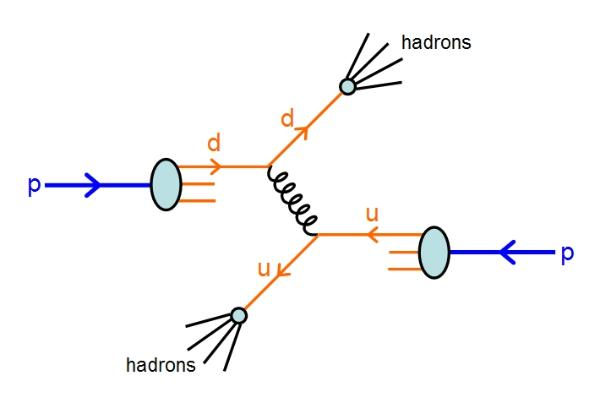
\includegraphics[clip,width=0.35\textwidth]{figuras/Chapter4/QCD}
   \caption{
  Schematic view of a di-jet production process that can fake the \Zprimetotauh~signature.
   }
   \label{fig:backgroundQCD}
\end{center}
\end{figure}


\item \textbf{Drell-Yan process ($pp \rightarrow \gamma^{*}/Z \rightarrow$ \tauh\tauh):}
Other background contribution comes from Drell-Yan processes in which the 
tau pair comes from the $\gamma^{*}/Z \rightarrow$ \tauh\tauh~decay. Since it has 
the same signatures than the signal this background is irreducible, in other words,
no topological criteria can be applied in order to suppress its contribution. However, this 
background can be distinguished from the signal, using the invariant mass distribution:
the $\gamma^{*}/Z \rightarrow$ \tauh\tauh~process has a mass peak is in the low 
region of the invariant mass distribution ($m(\tau_{1}, \tau_{2}) < 100$ \GeV), while the new resonance 
is expected in the high mass region. The properties of the Drell-Yan processes are
known to a high degree of accuracy and, indeed, the $\gamma^{*}/Z \rightarrow$ \tauh\tauh~events
are used to validate the tau identification criteria in 
the analysis (see section \ref{subsec:DY}). Figure \ref{fig:DY} shows the Feynman 
diagram for the Drell-Yan process production.

\begin{figure}[ht]
 \begin{center} 
 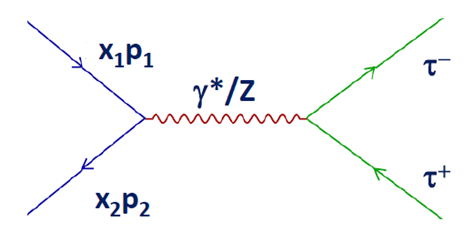
\includegraphics[clip,width=0.4\textwidth]{figuras/Chapter4/Background1}
 \caption{
  Feynman diagram for the $\gamma^{*}/Z \rightarrow$ \tauh\tauh~process.
   }
   \label{fig:DY}
\end{center}
\end{figure}

\item \textbf{W+Jets events:} The production of a W boson in association with 
jets (W+jets) can fake the signal events since the W decays 11.4$\%$
of the times into a tau plus a neutrino ($W\rightarrow \tau_{h} \nu_{\tau}$), 
while a jet can be misidentified as a hadronic tau; if such jet is in the 
opposite hemisphere than the W decay products, it would result into 
fake back-to-back \tauh\tauh~signal with a momentum imbalance due to the neutrino. 
Similarly, W+Jets can mimic the signal when the W boson 
decays hadronically (faking the \tauh~signature) and the jet (misidentified
as a tau) is produced in the opposite direction; however, the last scenario
can be suppressed since it does not have an intrinsic momentum imbalance. 
The W+Jets background contribution depends strongly 
on the jet $\rightarrow$ \tauh fake rate and, therefore, it can be highly reduced 
through the tau identification criteria. The W+Jets events represent 
7$\%$ of the total background contribution. Figure \ref{fig:WJets} shows the Feynman 
diagram for the W+Jets production process.

\begin{figure}[ht]
 \begin{center}
 \captionsetup[subfloat]{farskip=0pt,captionskip=0.0cm,labelformat=empty}
 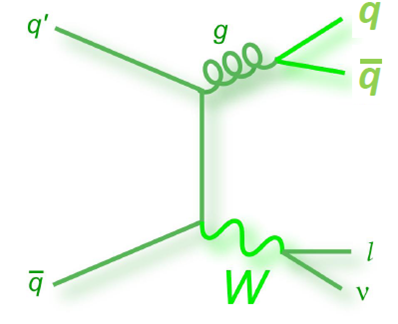
\includegraphics[clip,width=0.35\textwidth]{figuras/Chapter4/Background2}
 \caption{
  Feynman diagram for the W$+$Jet~process.
   }
 \label{fig:WJets}
\end{center}
\end{figure}

% \item \textbf{$b\bar{b}$ production:}

% Because b quarks can decay to muons
% (b → ν μ μc), QCD dijet backgrounds are mostly dominated by cases where bb̄ pairs
% are produced

% The case of the bb̄ production is important since b quarks decay into muons (b → ν μ μc), therefore
% the detector could identify one of the b-jets as a τ -jet and, on the other hemisphere, select the muon
% produced by the second b, faking the expected μτ h signal.

% The top (t) and anti-top (t) quarks decay primarily to a bottom quark (b)
 % or an anti-bottom (b) respectively through the emission of a W boson. This
% process produces signatures similar to the Z 0 → τ τ → eτ decay: the hadronic
% % W boson decay can look like a tau jet and the semielectronic decay can look
% like the semielectronic decay of a tau. Also, the W boson can decay to a tau
% % and a tau neutrino that can mimic the leptonic or hadronic tau from the Z 0
% decay. The associated jets from the b or b quarks hadronization though tend to
% produce a lot of extra particles that are used to identify this background. The
% b-tagging algorithm used to eliminate tt events is described in Section VII.6.

% \begin{figure}[ht]
%  \begin{center}
%  \captionsetup[subfloat]{farskip=0pt,captionskip=0.0cm,labelformat=empty}
%  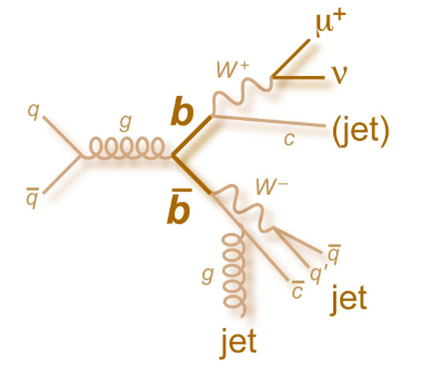
\includegraphics[clip,width=0.4\textwidth]{figuras/Chapter4/Background4}
% \end{center}
% \end{figure}

\item \textbf{$t\bar{t}$ production:} Another background comes from
the top-antitop production. The top quark decays most of the times into a
bottom quark and a W boson ($t\rightarrow Wb$). As in the case 
of the W+Jets, the W can result into a genuine tau coming from 
the $W\rightarrow \tau_{h} \bar{\nu}_{\tau}$ decay, or a fake tau 
coming from its hadronic decay. Therefore, each W boson, that comes 
from the top and the antitop decays, can mimic the di-hadronic tau 
signature with a momentum imbalance due to the presence of neutrinos. Additionally, 
the b quark coming from the top decay can result into a hadronic 
jet, which can fake the \tauh~signature. This background is highly suppressed
through the rejection of any jet identified as a b-jet; with this purpose, the b-tagging algorithm
described in section \ref{sec:bJet} is used. The $t\bar{t}$ production represents 
less than $1\%$ of the total background. Figure \ref{fig:ttbar} shows the Feynman 
diagram for the $t\bar{t}$ production process.

\begin{figure}[ht]
 \begin{center} \label{fig:ttbar}
 \captionsetup[subfloat]{farskip=0pt,captionskip=0.0cm,labelformat=empty}
 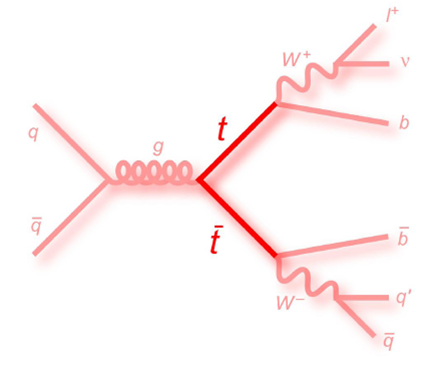
\includegraphics[clip,width=0.4\textwidth]{figuras/Chapter4/Background5}
 \caption{
  Feynman diagram for the top-antitop~production.
   }
 \label{fig:ttbar}
\end{center}
\end{figure}

\item \textbf{Di-Boson processes:} The di-boson background refers to 
the $ZZ$, $WZ$, and $WW$ production. As was mentioned above, 
both, Z and W bosons, can result into a genuine or a fake tau 
in the final state. This background accounts
for all the possible combinations of tau pairs, 
coming from the di-boson processes. The tau pairs 
 can mimic the topological features of the signal. The di-bosons 
 SM process does not have a significant contribution 
 to the total background (less than 1$\%$). Figure \ref{fig:DiBoson} shows the Feynman 
diagram for the di-boson production process.

\begin{figure}[ht]
 \begin{center}
 \captionsetup[subfloat]{farskip=0pt,captionskip=0.0cm,labelformat=empty}
 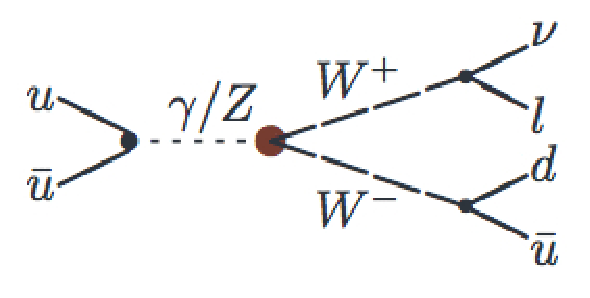
\includegraphics[clip,width=0.35\textwidth]{figuras/Chapter4/BackgroundDibosonWW}
 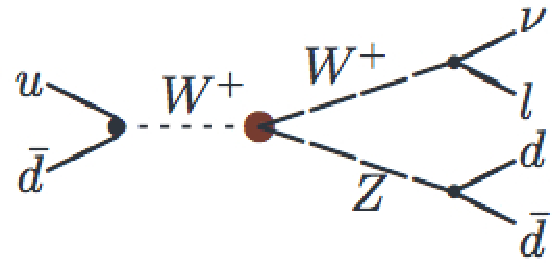
\includegraphics[clip,width=0.35\textwidth]{figuras/Chapter4/BackgroundDibosonWZ}
 \caption{
  Feynman diagrams of two scenarios of di-boson production that can fake the \Zprimetotauh~signature.
   }
 \label{fig:DiBoson}
\end{center}
\end{figure}

\item \textbf{H $\rightarrow$ \tauh\tauh~process:} the Higgs boson can decay 
into two-hadronic taus and, similarly to the Drell-Yan case, this background has the same 
topology than the signal. However, the contribution from H $\rightarrow$ \tauh\tauh~is 
not significant since the events lie in the low region of the invariant mass 
distribution. Also, in contrast with the Drell Yan process, it has a small
production cross section. The H $\rightarrow$ \tauh\tauh~process only represents
the 0.035$\%$ of the total background in the signal region.
\end{itemize}

\noindent In summary, the dominant background for the \Zprimetotauh~signature
comes from the QCD multi-jet events, which correspond to around 70$\%$ of the 
total; this background can be reduced since it does not 
have the momentum imbalance of the signal. The other important background comes from 
Drell-Yan processes, which have the same signature than the signal with exception
of the low invariant mass of the decay products; this background is known 
with a high degree of accuracy and  it can be used to validate the tau 
identification criteria used in this analysis. The remaining backgrounds,
W+Jets, $t\bar{t}$ and di-boson, can be reduced through tau identification criteria and 
topological event selections, and they represent 8$\%$ of the total background. The 
$\textrm{H} \rightarrow \tau_{h}\tau_{h}$ background is not considered in this analysis since
its contribution is negligible ($0.035\%$).

\section{Mass Reconstruction}
\label{sec:Mass Reconstruction}

As has been mentioned, if a \Zprime~boson exists, it would be observed
as a peak in the invariant mass distribution of its decay products 
and, therefore, the search for this new boson consists on distinguishing this
heavy resonance from the background processes that lie in the low mass region. In the particular 
\Zprimetotautau~case, it is not possible to reconstruct fully the di-tau invariant mass
due to the presence of neutrinos in the final state (see section \ref{sec:RecoTau}). In consequence,
a narrow peak will not be observed and, instead, the \Zprime~events would manifest them selves
as an enhanced mass above the expected level of background. Nevertheless, in order to 
consider the unmeasured energy of the neutrinos, the missing transverse energy can be 
included in the mass calculation. A $M(\tau_1,\tau_2,\not\!\!E_T)$ variable, known as the \textit{effective visible mass},
defined as:

\begin{equation} \label{eq:eff_mass}
M(\tau_1,\tau_2,\not\!\!E_T)  = \sqrt{(E_{\tau_1} + E_{\tau_2} + \not\!\!E_T)^2 - (\vec{p}_{\tau_1} + \vec{p}_{\tau_2} + \not\!\!\vec{E}_T)^2} \;, \\
\end{equation}

\noindent includes the intrinsic missing transverse energy of the \Zprimetotautau~events and, therefore,
allows an improved discrimination of the signal against the backgrounds when compared with 
the simple invariant mass variable. In summary, the search for \Zprimetotauh~events 
reduces to the the search for enhanced heavy resonances in the $M(\tau_1,\tau_2,\not\!\!E_T)$ distribution 
of the di-hadronic tau decay products. Figure \ref{eq:Zprime_mass_distribution}
shows the $M(\tau_1,\tau_2,\not\!\!E_T)$ distribution of the di-hadronic final state
for the expected background and a MC signal sample with an expected mass of 3 \TeV. As can be 
seen in the figure, most of the backgrounds lie in the low mass region of the mass spectrum, while the 
expected signal is located in the high mass region.

\section{Strategy}
\label{sec:Strategy}

Since a \Zprime~is a neutral and massive boson, we look for 
two oppositely-charged taus with high transverse momentum, that 
travel in opposite directions. As was mentioned above, the signal events must
have missing transverse energy, due to the presence of neutrinos. An event selection 
is performed according to these topological features, 
in order to identify the signal with high efficiency; additionally, these
selection criteria allow to optimize the rejection of any background 
process that can mimic the signal, reducing the influence of systematic 
uncertainties. \\

\noindent The discrimination between signal and background events is performed
using the effective visible mass variable, since the \Zprimetotauh~events 
would give high values and the background processes would give low values. In order 
to interpret the data and to extract any possible excess from the 
SM expectation, or to establish exclusion limits, a statistical 
analysis, based on binned likelihood functions, was implemented. In 
chapter \ref{chap:Analysis}, the whole analysis is presented, starting from the 
description of the data sets, the event selection, the estimation of background 
and the systematic effects.

\begin{figure}[H]
 \begin{center}
 \captionsetup[subfloat]{farskip=0pt,captionskip=0.0cm,labelformat=empty}
 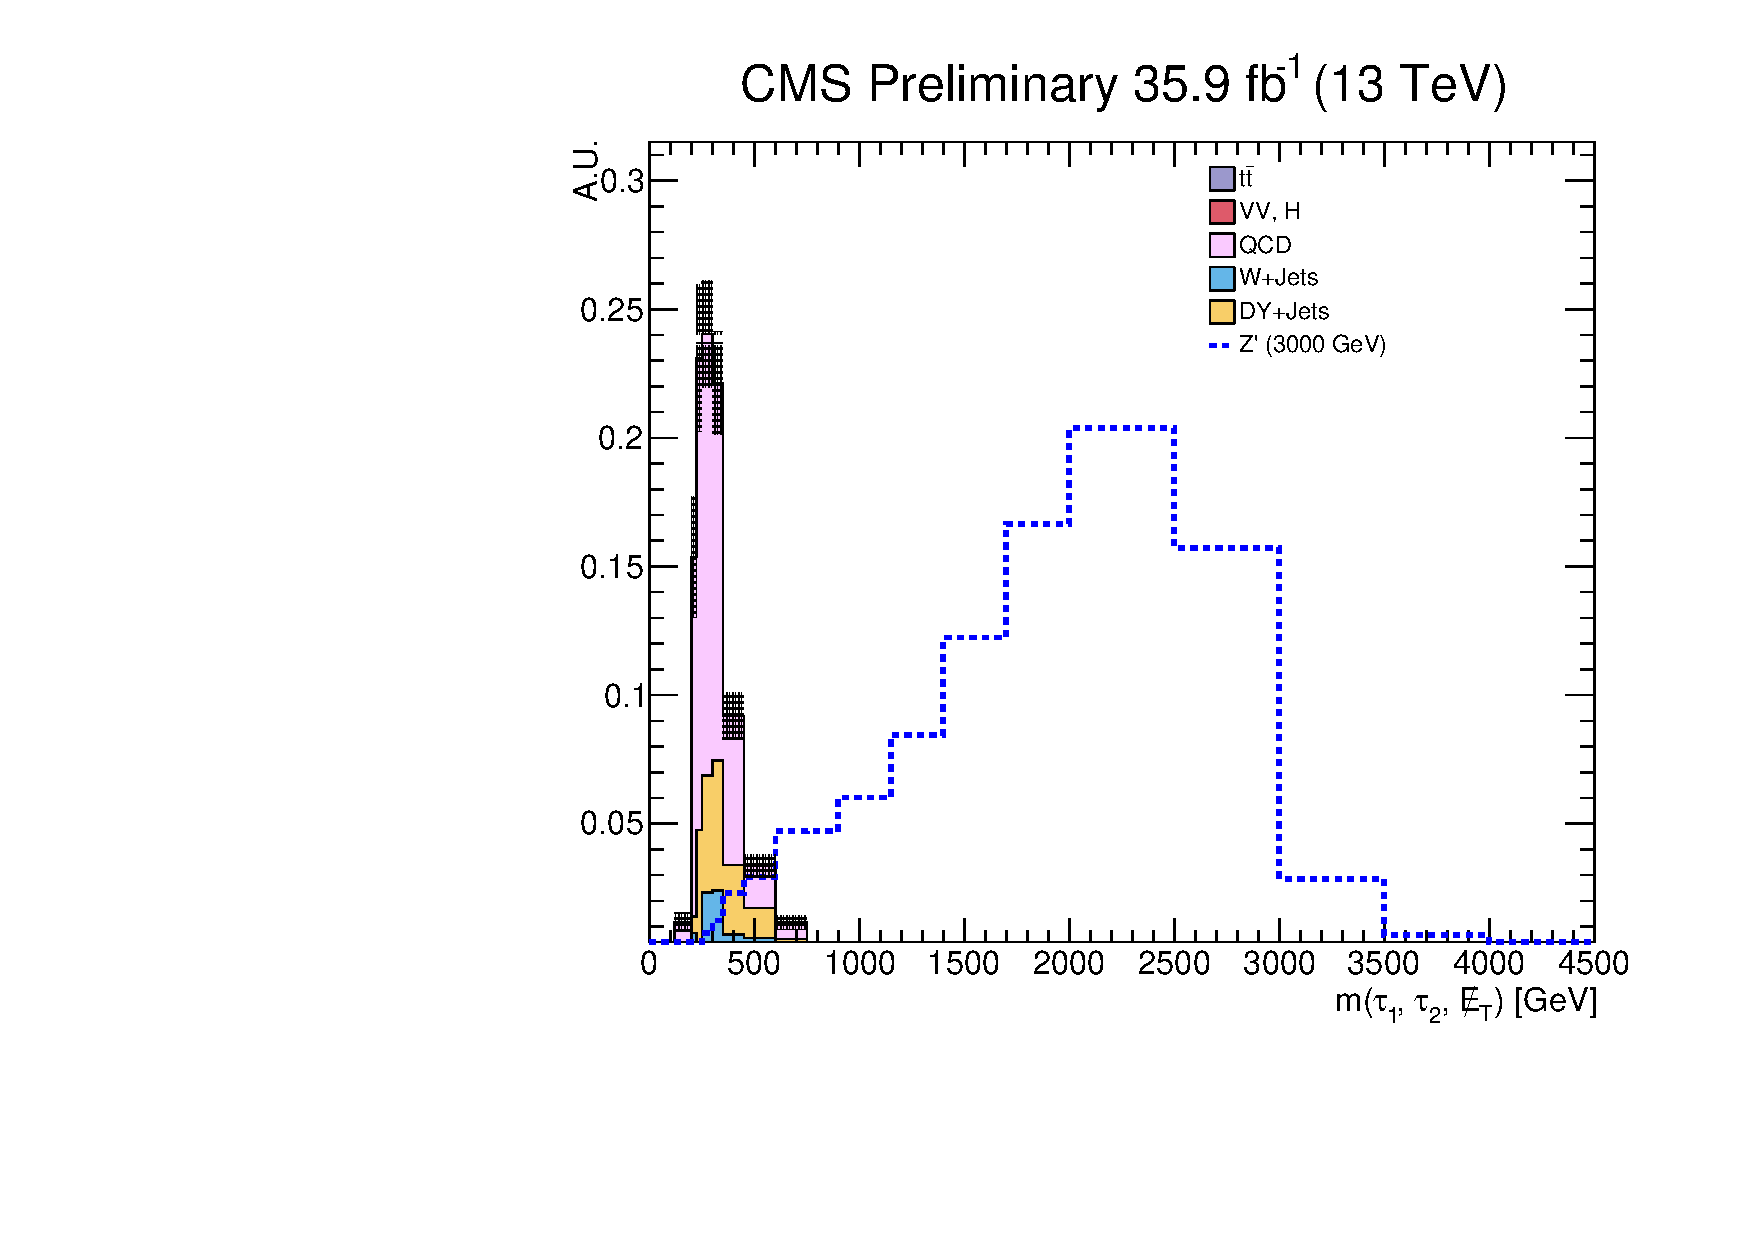
\includegraphics[clip,width=0.5\textwidth]{figuras/Chapter4/EffVisibleMass_unity.pdf}
\caption{  $M(\tau_1,\tau_2,\not\!\!E_T)$  distribution of di-hadronic tau 
final state for the expected backgrounds and 
a \Zprime~signal with an expected mass of 3 \TeV. The 
distribution was obtained from the events that have passed 
the selection criteria described in section \ref{sec:EventSelection}.The background 
estimation was performed according the the method described in section \ref{sec:BackgroundEstimation}. 
}
\label{eq:Zprime_mass_distribution}
 \end{center}
\end{figure}